% rhombicuboctahedron wireframe: V=24 E=48 F=26 (8 triangles + 18 squares),
% orthographic projection Rx=10 Ry=-12, solid=front/silhouette, dashed=hidden.
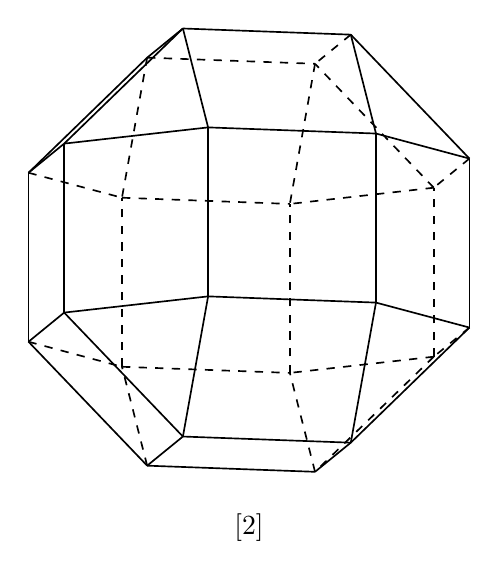
\begin{tikzpicture}[x=1mm,y=1mm,line width=.6pt,font=\normalsize]
\tikzset{hidden edge/.style={dashed}}
\draw (-23.47,-7.93) -- (-28.00,-11.63);
\draw (-23.47,-7.93) -- (-23.47,13.53);
\draw (-23.47,-7.93) -- (-8.39,-23.67);
\draw (-23.47,-7.93) -- (-5.19,-5.87);
\draw (-28.00,-11.63) -- (-28.00,9.83);
\draw (-28.00,-11.63) -- (-12.93,-27.37);
\draw (-23.47,13.53) -- (-28.00,9.83);
\draw (-23.47,13.53) -- (-8.39,28.15);
\draw (-23.47,13.53) -- (-5.19,15.59);
\draw (-28.00,9.83) -- (-12.93,24.45);
\draw (28.00,-9.83) -- (28.00,11.63);
\draw (28.00,-9.83) -- (12.93,-24.45);
\draw (28.00,-9.83) -- (16.13,-6.66);
\draw (28.00,11.63) -- (12.93,27.37);
\draw (28.00,11.63) -- (16.13,14.81);
\draw (-8.39,-23.67) -- (-12.93,-27.37);
\draw (-8.39,-23.67) -- (12.93,-24.45);
\draw (-8.39,-23.67) -- (-5.19,-5.87);
\draw (-12.93,-27.37) -- (8.39,-28.15);
\draw (-8.39,28.15) -- (-12.93,24.45);
\draw (-8.39,28.15) -- (12.93,27.37);
\draw (-8.39,28.15) -- (-5.19,15.59);
\draw (12.93,-24.45) -- (8.39,-28.15);
\draw (12.93,-24.45) -- (16.13,-6.66);
\draw (12.93,27.37) -- (16.13,14.81);
\draw (-5.19,-5.87) -- (-5.19,15.59);
\draw (-5.19,-5.87) -- (16.13,-6.66);
\draw (-5.19,15.59) -- (16.13,14.81);
\draw (16.13,-6.66) -- (16.13,14.81);
\draw[hidden edge] (-28.00,-11.63) -- (-16.13,-14.81);
\draw[hidden edge] (-28.00,9.83) -- (-16.13,6.66);
\draw[hidden edge] (28.00,-9.83) -- (23.47,-13.53);
\draw[hidden edge] (23.47,-13.53) -- (23.47,7.93);
\draw[hidden edge] (23.47,-13.53) -- (8.39,-28.15);
\draw[hidden edge] (23.47,-13.53) -- (5.19,-15.59);
\draw[hidden edge] (28.00,11.63) -- (23.47,7.93);
\draw[hidden edge] (23.47,7.93) -- (8.39,23.67);
\draw[hidden edge] (23.47,7.93) -- (5.19,5.87);
\draw[hidden edge] (-12.93,-27.37) -- (-16.13,-14.81);
\draw[hidden edge] (-12.93,24.45) -- (8.39,23.67);
\draw[hidden edge] (-12.93,24.45) -- (-16.13,6.66);
\draw[hidden edge] (8.39,-28.15) -- (5.19,-15.59);
\draw[hidden edge] (12.93,27.37) -- (8.39,23.67);
\draw[hidden edge] (8.39,23.67) -- (5.19,5.87);
\draw[hidden edge] (-16.13,-14.81) -- (-16.13,6.66);
\draw[hidden edge] (-16.13,-14.81) -- (5.19,-15.59);
\draw[hidden edge] (-16.13,6.66) -- (5.19,5.87);
\draw[hidden edge] (5.19,-15.59) -- (5.19,5.87);
\node[anchor=north] at (0,-32.15) {\bitmapinsertcaption[2]};
\end{tikzpicture}
